\section{bpred\_\-perfect\_\-t Class Reference}
\label{classbpred__perfect__t}\index{bpred\_\-perfect\_\-t@{bpred\_\-perfect\_\-t}}
Inheritance diagram for bpred\_\-perfect\_\-t:\nopagebreak
\begin{figure}[H]
\begin{center}
\leavevmode
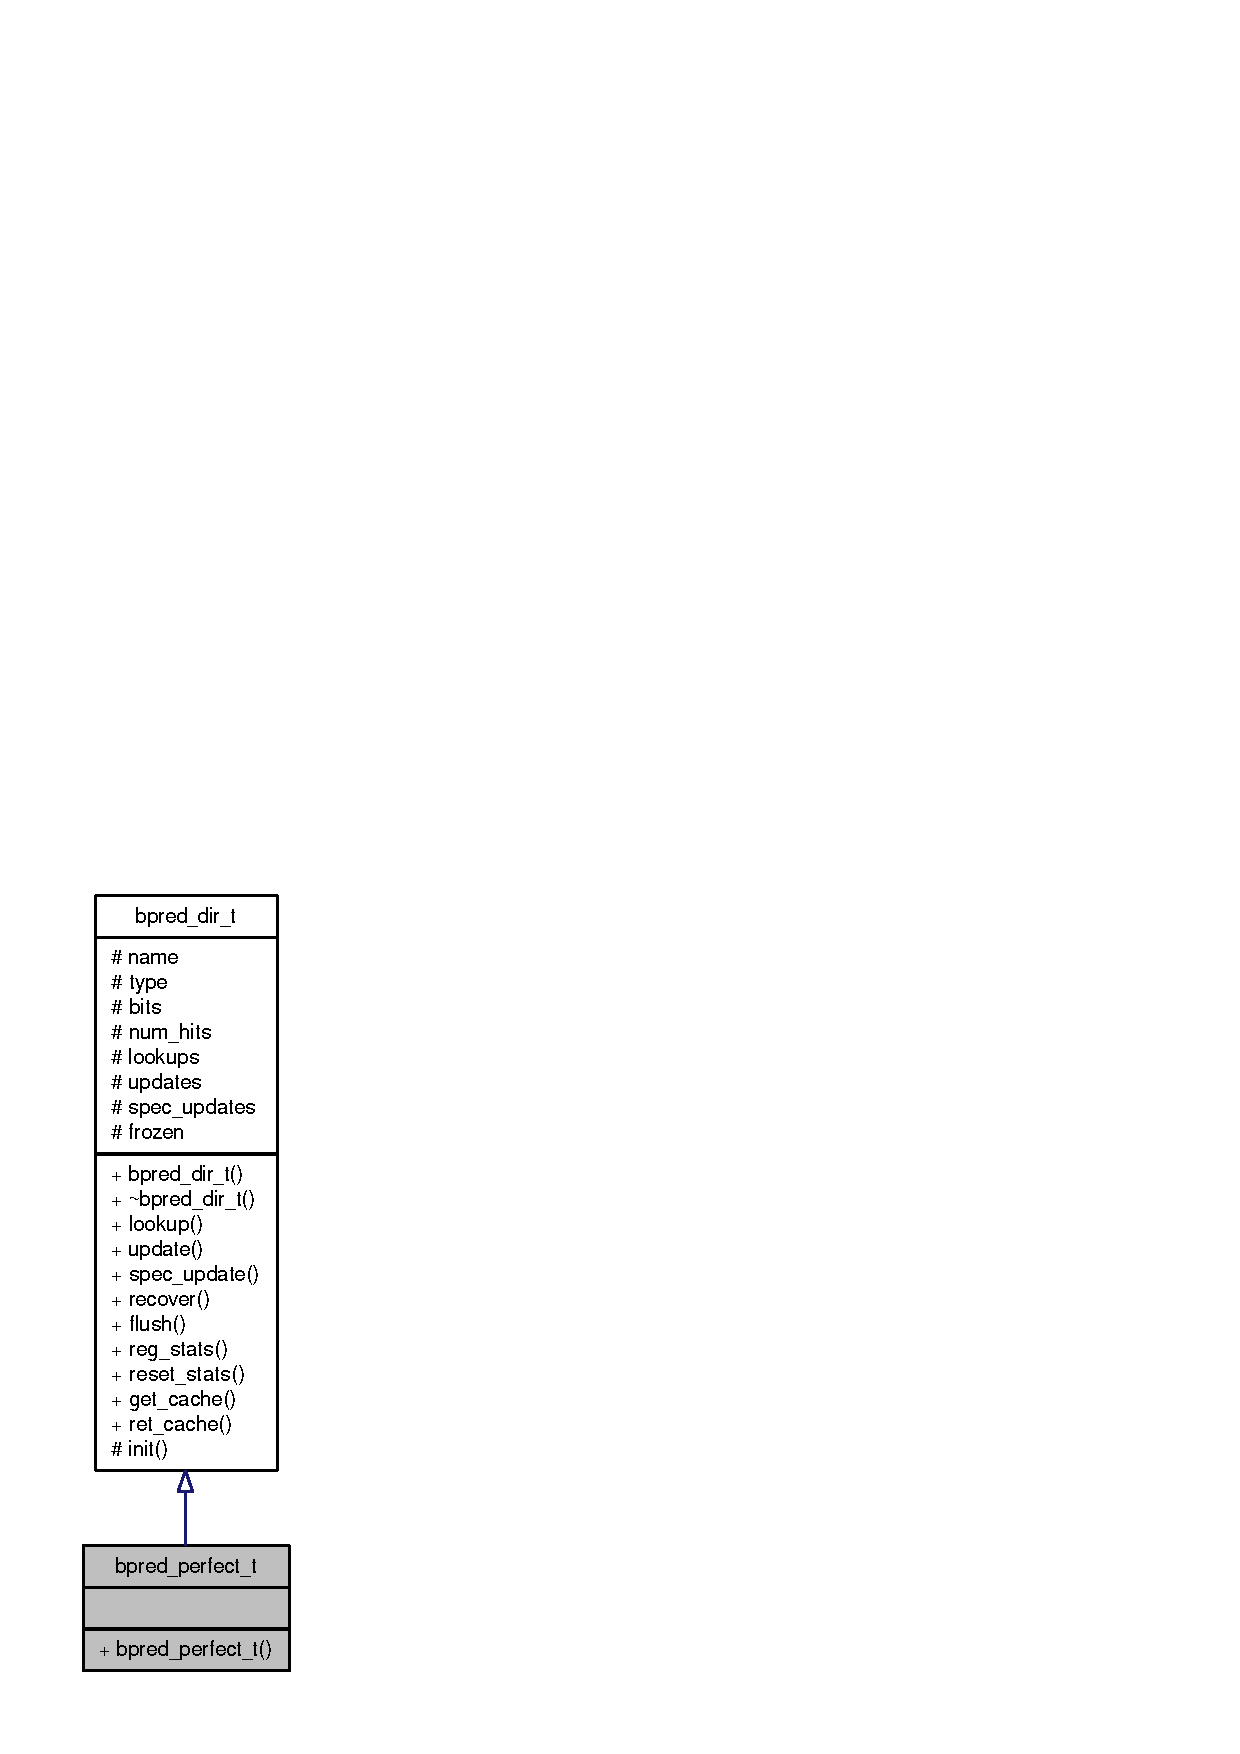
\includegraphics[height=400pt]{classbpred__perfect__t__inherit__graph}
\end{center}
\end{figure}
Collaboration diagram for bpred\_\-perfect\_\-t:\nopagebreak
\begin{figure}[H]
\begin{center}
\leavevmode
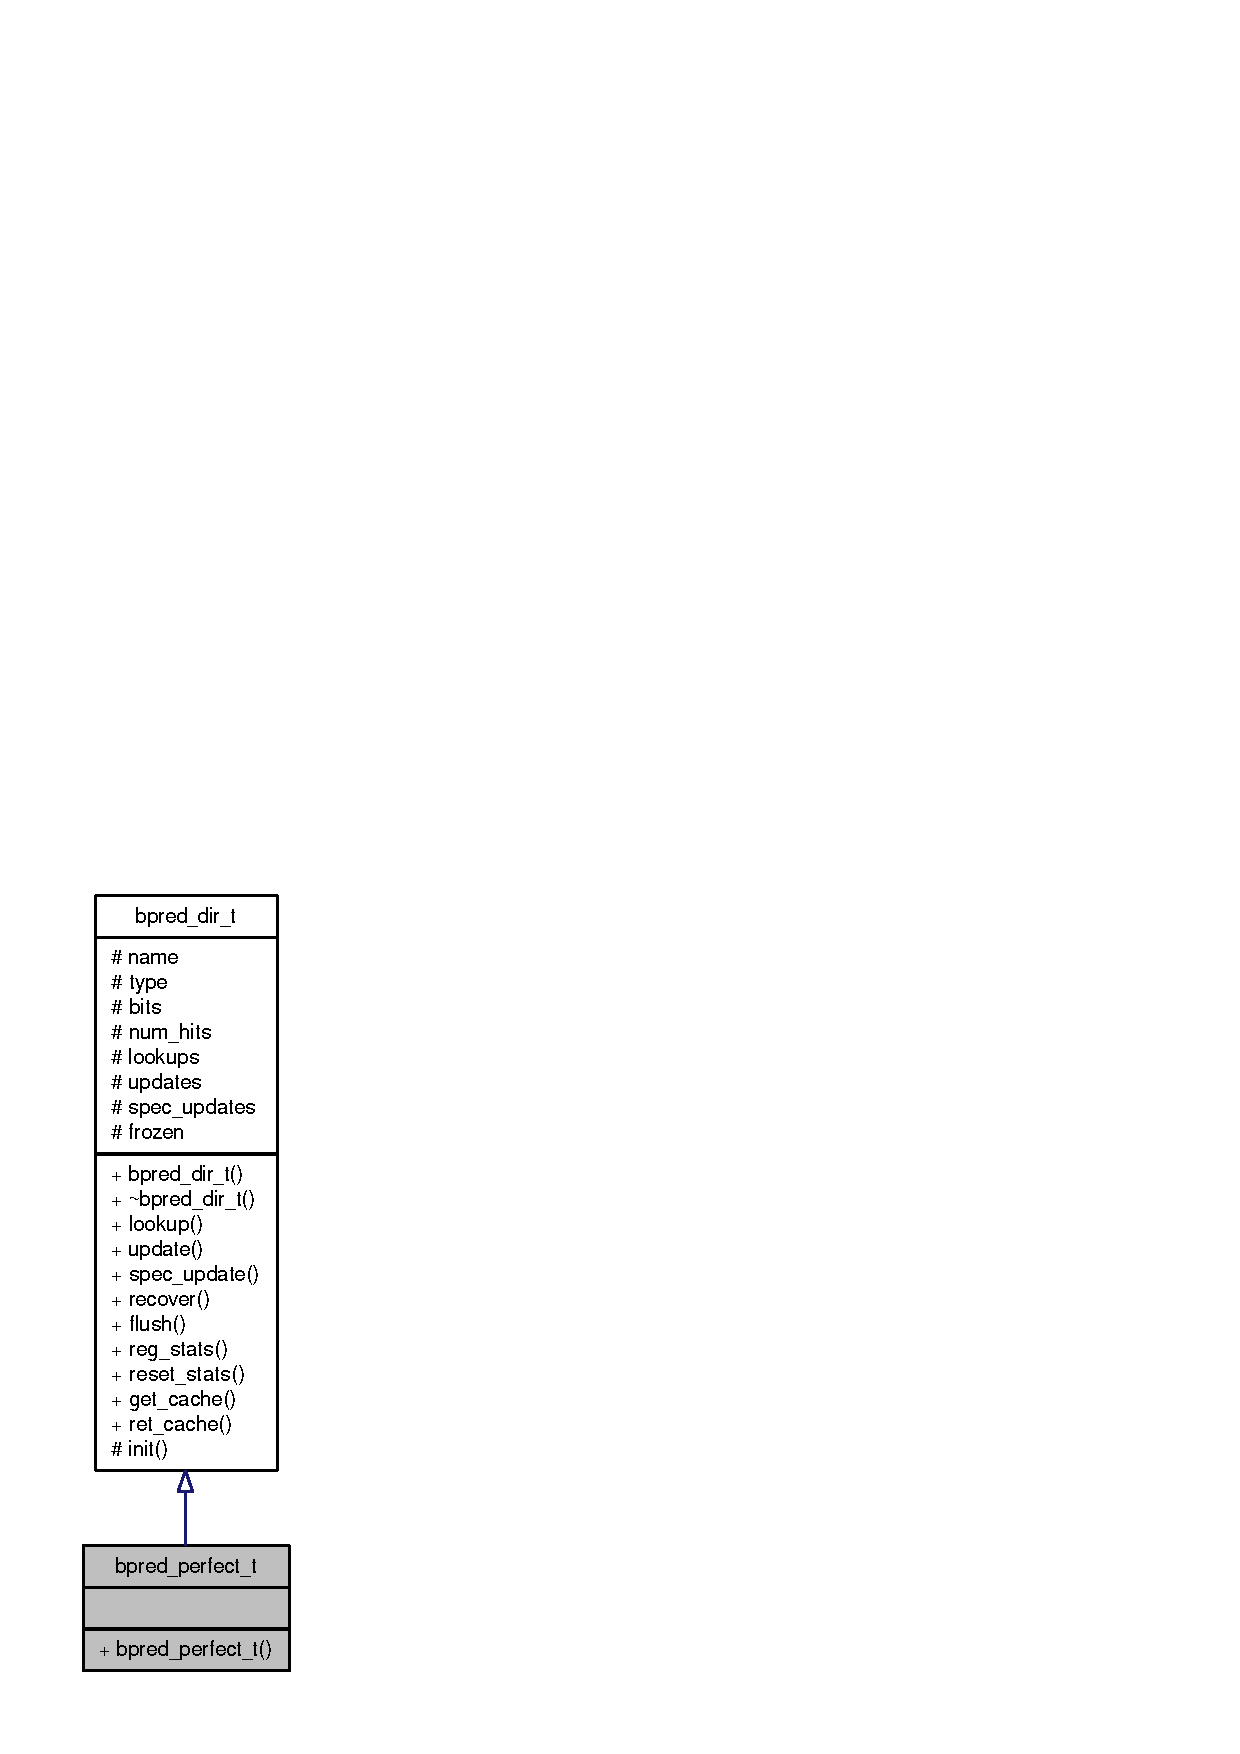
\includegraphics[height=400pt]{classbpred__perfect__t__coll__graph}
\end{center}
\end{figure}
\subsection*{Public Member Functions}
\begin{CompactItemize}
\item 
{\bf bpred\_\-perfect\_\-t} ()
\end{CompactItemize}


\subsection{Detailed Description}


Definition at line 16 of file bpred-perfect.cpp.

\subsection{Constructor \& Destructor Documentation}
\index{bpred\_\-perfect\_\-t@{bpred\_\-perfect\_\-t}!bpred\_\-perfect\_\-t@{bpred\_\-perfect\_\-t}}
\index{bpred\_\-perfect\_\-t@{bpred\_\-perfect\_\-t}!bpred_perfect_t@{bpred\_\-perfect\_\-t}}
\subsubsection[{bpred\_\-perfect\_\-t}]{\setlength{\rightskip}{0pt plus 5cm}bpred\_\-perfect\_\-t::bpred\_\-perfect\_\-t ()\hspace{0.3cm}{\tt  [inline]}}\label{classbpred__perfect__t_b3156d0207bb3614428e0d874d6bb69a}




Definition at line 20 of file bpred-perfect.cpp.

References bpred\_\-dir\_\-t::bits, COMPONENT\_\-NAME, fatal(), bpred\_\-dir\_\-t::init(), bpred\_\-dir\_\-t::name, and bpred\_\-dir\_\-t::type.

The documentation for this class was generated from the following file:\begin{CompactItemize}
\item 
{\bf bpred-perfect.cpp}\end{CompactItemize}
